\section{Implementation architecture}

In this chapter, we discuss the implementation details of the Train Benchmark. The installation guide is available in the MONDO wiki.\footnote{\url{https://opensourceprojects.eu/p/mondo/wiki/TrainBenchmark/}}

%\section{Architecture}

For the integration of the Train Benchmark projects and their third party dependencies, we use Apache Maven~\cite{Maven}. The dependencies are shown in \figref{fig:trainbenchmark-modules}.

\begin{figure}%[!htb]
	\centering
	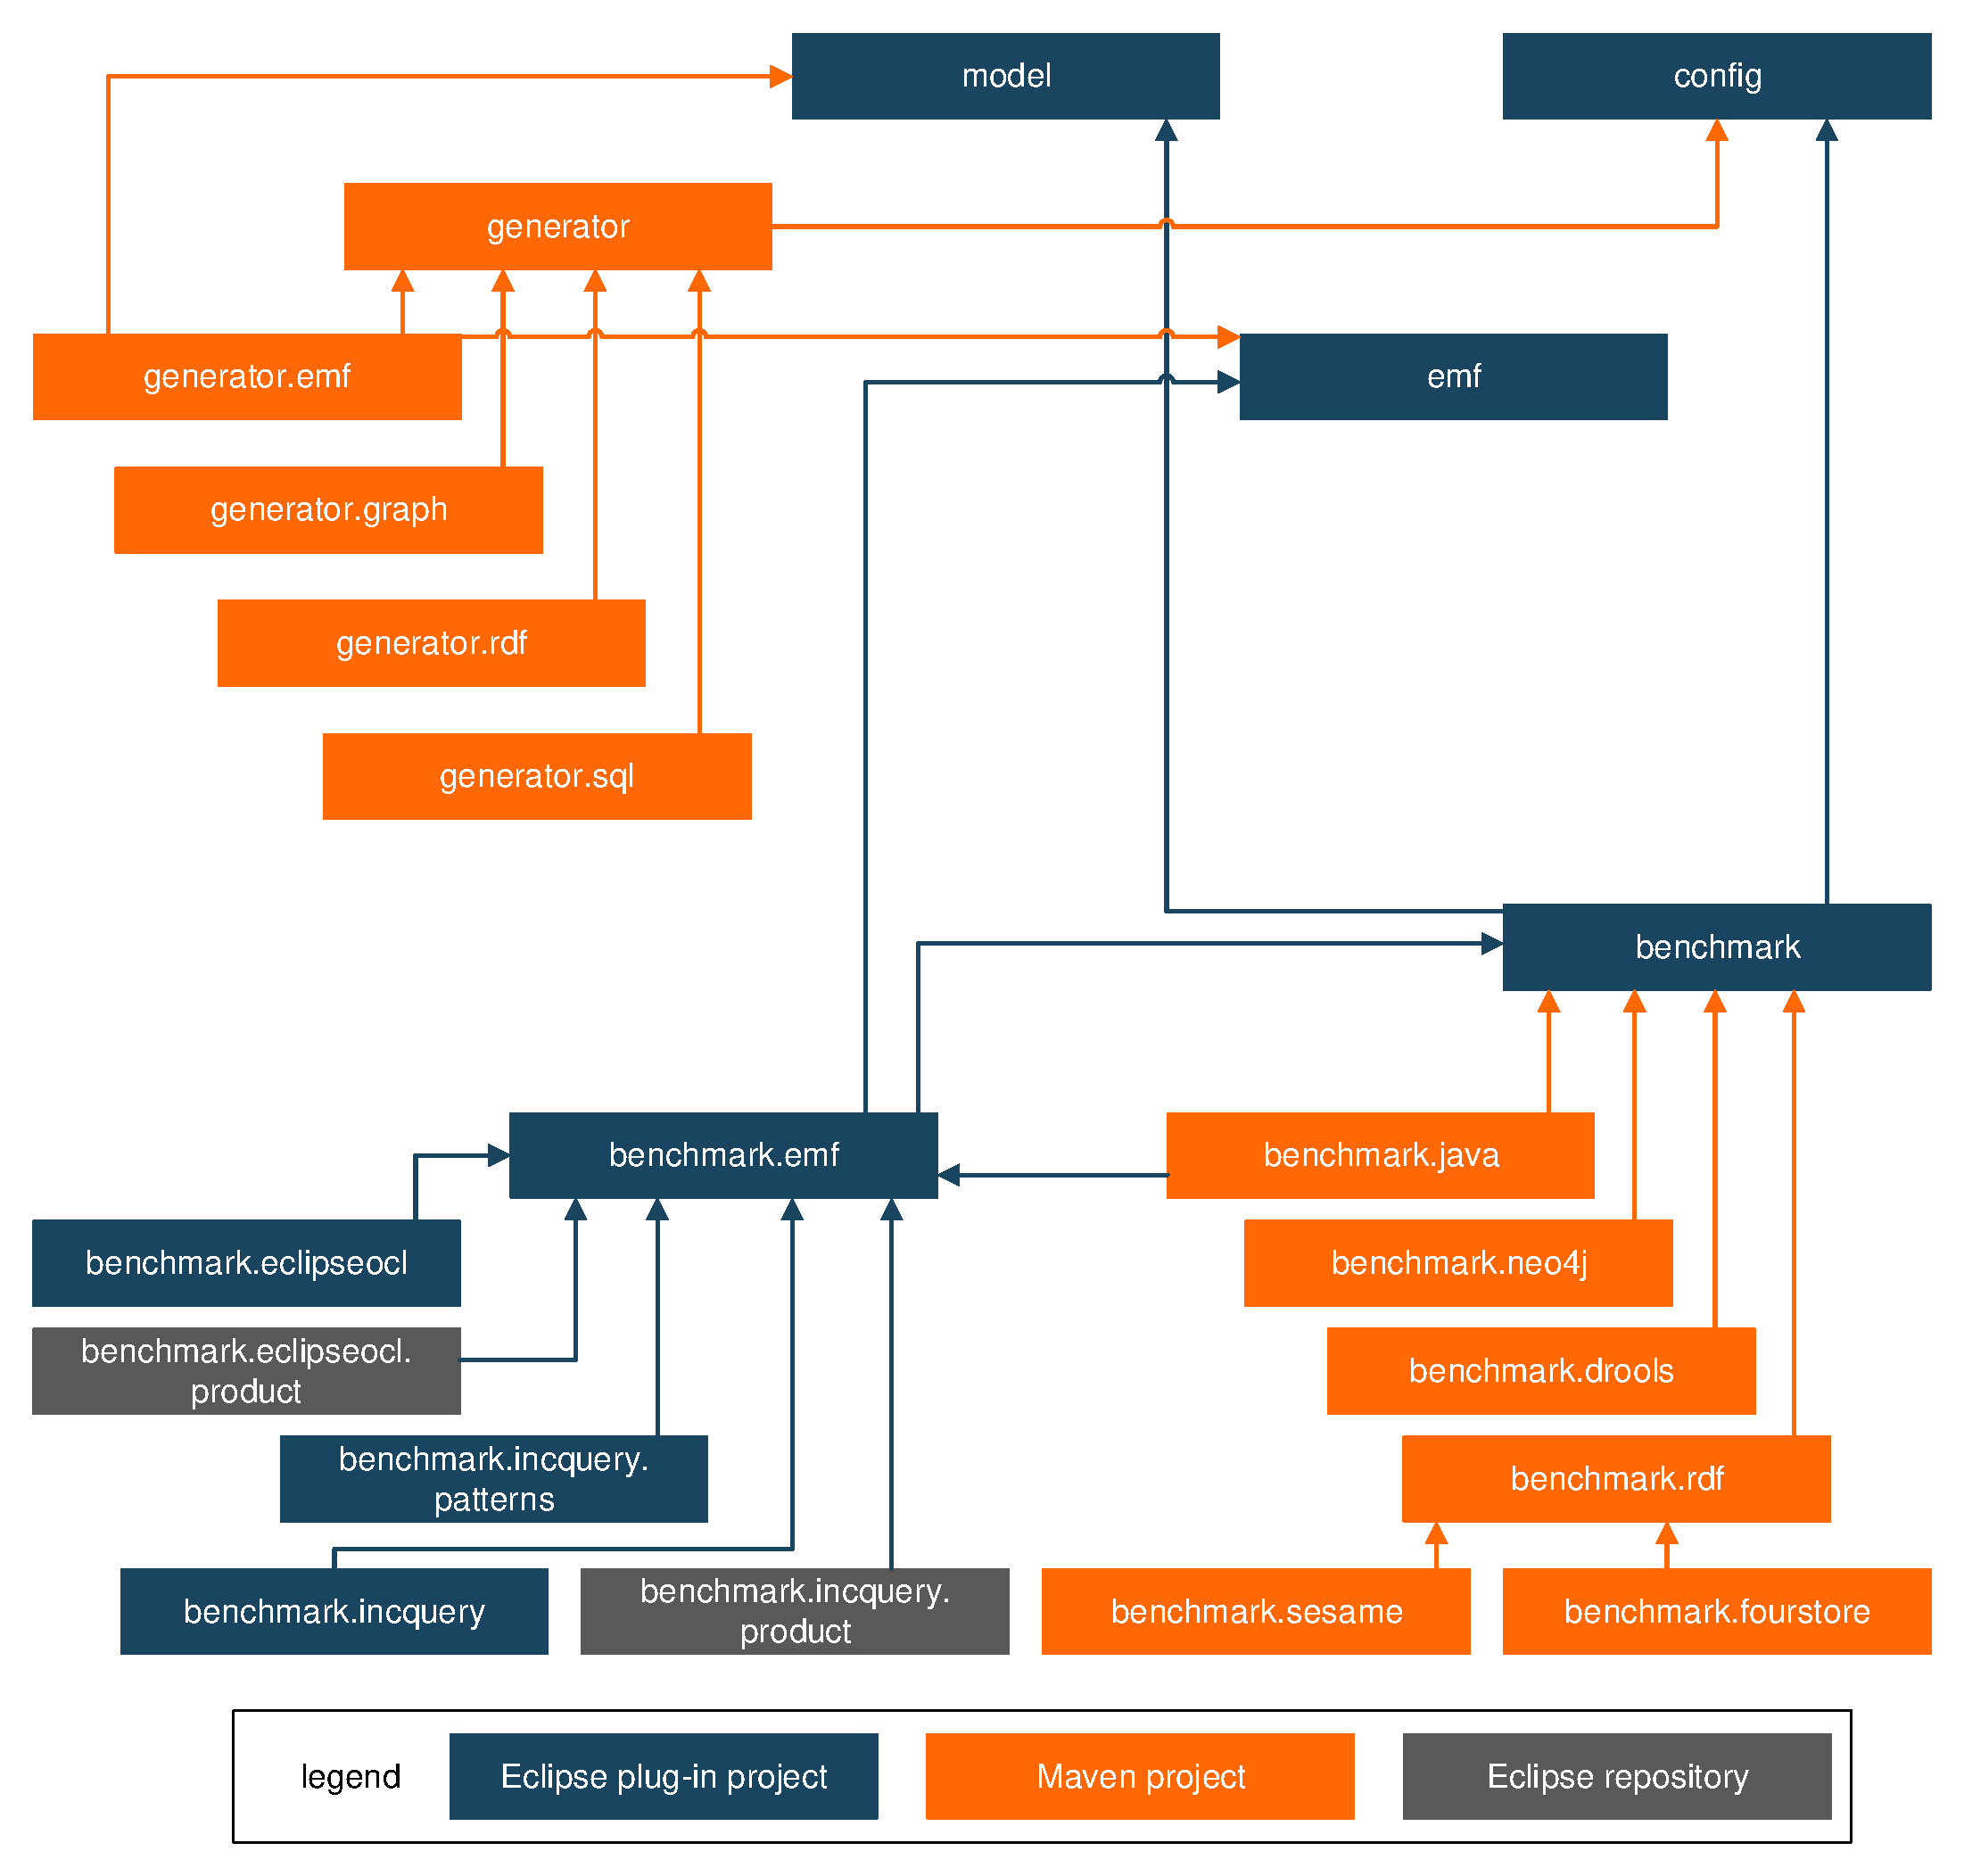
\includegraphics[width=\textwidth]{figures/trainbenchmark-modules}
	\caption{The Maven modules defined in the Train Benchmark. Note that artifact ids of the modules are shortened and the full ids start with \texttt{hu.bme.mit.trainbenchmark}.}
	\label{fig:trainbenchmark-modules}
\end{figure}

In this section, we briefly describe the tasks and responsibilities of each module.

\subsection{Parent module}

The \texttt{hu.bme.mit.trainbenchmark} module is the parent module which contains the modules used in the Train Benchmark. Building this Maven module builds all child modules as well.

\subsection{Central modules}

The \texttt{hu.bme.mit.trainbenchmark.model} module contains the reference metamodel represented in EMF.

The \texttt{hu.bme.mit.trainbenchmark.config} module contains classes and constants used by the \texttt{generator} and the \texttt{benchmark} projects.

\subsection{Representation-specific modules}

The \texttt{hu.bme.mit.trainbenchmark.emf} and \texttt{hu.bme.mit.trainbenchmark.rdf} modules contain classes and constants used by the particular representations.

\subsection{Generator modules}

The \texttt{hu.bme.mit.trainbenchmark.generator.*} modules are responsible for generating the instance models for the benchmarks.

\begin{itemize}
  \item \texttt{emf}: generates an EMF instance model.
  \item \texttt{emfuuid}: generates an EMF instance model with UUIDs. A UUID (universally unique identifier) identifies an EObject uniquely, and is generated automatically by the EMF framework. In the output file, UUIDs are used to reference other objects, and not XPath expressions, speeding up the serialization process.
  \item \texttt{graph}: generates a property graph model in the specified format: GraphML (default), Blueprints GraphSON, Faunus GraphSON.
  \item \texttt{rdf}: generates an RDF instance model.
  \item \texttt{sql}: generates an SQL script which creates and loads the appropriate database tables.
\end{itemize}


\subsection{Benchmark modules}

The \texttt{hu.bme.mit.trainbenchmark.benchmark.*} modules are responsible for benchmarking. For the list of current implementations, see \autoref{tbl:tools}.

\subsection{4store}

To access 4store through a graph-like API, we developed a Java client with a focus on high performance.

\begin{itemize}
  \item Homepage: \url{https://git.inf.mit.bme.hu/w?p=projects/bigmodel/4store-graph-client.git}
  \item Clone URI: \url{https://anonymous@git.inf.mit.bme.hu/r/projects/bigmodel/4store-graph-client.git}
\end{itemize}

%\subsection{Extending the framework with custom tools, queries or models}
%\subsubsection{Extending the model generator with new syntaxes}
%\subsubsection{Adding a tool to measure performance}
